\chapter{Dual-Zone: Day/Night Zoning}
\label{ch:cs1}

In order to evaluate the effectiveness of MacroLab as a CPS macroprogramming
abstraction and to get a better understanding of the weaknesses of
macroprogramming languages for CPS application development a complex sensing and
control application is necessary. An occupant-oriented HVAC control system is
such an application. This system is developed in three phases, each serving as a
case study used to evaluate MacroLab. Case study 1 discusses {\em Dual-Zone}: a
statically zoned system where a house is separated into two zones one of which
is conditioned at night while the other is conditioned during the day.

Even though static zoning is a simple approach, controlling such a system based
on occupancy could reduce wasted energy that is used to heat and cool unoccupied
rooms. However, the energy savings of such a system is not a foregone conclusion
due to three key challenges. First, the size of the HVAC system is typically
chosen based on the size of the entire house, and so heating or cooling only a
fraction of the house with an oversized system for that fraction could prove
inefficient. Second, restricting airflow into some rooms will create
backpressure in the ducts, which can further reduce the efficiency of the HVAC
system by causing leaks in the ducts and at the dampers. Third, most houses do
not have insulated interior walls, and the lack of thermal insulation between
rooms can lead to heat transfer between the conditioned and unconditioned zones.

This case study demonstrates the feasibility of saving energy by retrofitting a
centralized HVAC system to be controlled as a two zoned system where one zone is
activated during the day while the other zone is activated at night. A wireless
sensor/actuator system that can be cheaply and easily deployed in existing homes
is implemented. The system includes 21 temperature sensors and a wireless
thermostat that controls the HVAC hardware and mechanically opens and closes
dampers in order to control airflow through the home. The components used cost
less than \$500, and a production version is expected to cost considerably
less. In contrast, traditional zoning systems often cost more that
\$5000. Dual-Zone zoning is deployed in a 7-room, single-story, 1400 square foot
house and measured the energy consumption of heating and cooling. The results
indicate that the system consumed 20.5\% less energy than if the HVAC system
were controlled by the existing thermostat over a 20-day experimental period
indicating that retrofitting an existing centralized HVAC system for day/night
zoning has a potential for substantial energy savings.

\section{Background and Related Work}
\label{sec:relatedWork}

Traditional HVAC zoning systems for homes typically separate a house into
floors, each of which can be controlled individually.  These systems are often
installed more for comfort than for energy savings, because a single un-zoned
system that operates on multiple floors will often result in a warm top floor
and/or a cold bottom floor.  Floor-level zoning also makes sense in many homes
that have bedrooms on the top floor and living areas on the bottom floor.
Floor-level systems have resulted in homeowners saving as much as 20-30\% as
compared to single zoned systems~\cite{Systems2003}. However, these systems are
expensive and the energy savings can take years or even decades to produce a
positive return on investment.  Furthermore, it can be difficult to retrofit an
existing home with a zoning system.

Numerous studies have explored the effect of zoning a centralized HVAC system,
but the results have been mixed and inconclusive.  One experiment tested the
energy used to heat a single-room with 10 registers and leaky ducts while
closing an increasing number of vent registers~\cite{walker2003register}.  The
results indicate that closing registers increases the pressure within ducts
causing greater duct leakage and reduced system efficiency.  However, since all
registers were within the same room, this study did not determine whether the
reduced efficiency outweighs the savings produced by conditioning a smaller
area; all register configurations were conditioning the same sized area.

A subsequent study developed an automated vent louver design for
zoning~\cite{watts2007application}, similar to the one developed for
day/night zoning and other similar systems~\cite{redfern2006design}.  The
authors evaluate the system by dividing a house in Danville, CA into four zones
and increase the temperature in each zone by 2-5$^\circ$ F. They also increased
the temperature in the entire house by the same amount.  The results indicate
that it takes less energy to increase the zone temperature per degree than it
takes to increase the whole house temperature per degree, since the smaller
zones heat up faster than the whole house, allowing the system to turn off
sooner.  However, this study only measured the transitional time and energy of a
zoned system, and it did not measure the steady state energy.  In other
words, it does not show the difference in energy required to {\em maintain} a
particular temperature in a zone versus the whole house.  This distinction is
profound, because thermal leakage between adjacent rooms could cause system to
also turn back on more quickly, nullifying the energy savings of turning off
more quickly.  This is often called {\em short cycling}, and is known to
decrease system efficiency as well as reduce the overall lifetime of the
equipment.

\section{Intuition and Preliminary Studies}
\label{sec:intuition}

\begin{figure}[t]
  \centering
  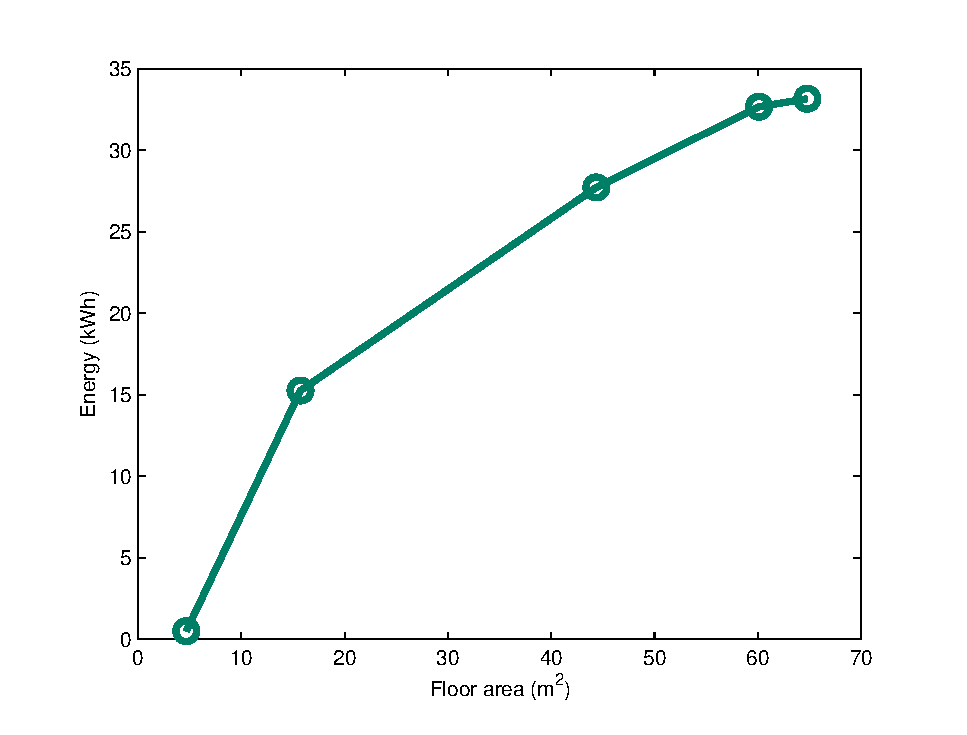
\includegraphics[width=0.6\columnwidth]{fig/areaVsEnergy}
  \caption[Effect of Floorspace on Energy Usage]{With an ideal system, the
    amount of energy used for conditioning a building is almost proportional to
    the floorspace being conditioned.}
  \label{fig:areaVsEnergy}
\end{figure}

Before implementing Dual-Zone, two simulation studies were performed to
better understand whether such a system should be expected to reduce energy
savings, and why. A third analysis of a publicly available smart home data
set~\cite{kasterenUbi2008} was carried out to verify that room usage frequencies
change throughout the day.  These three studies are explained in the following
subsections.

\subsection{Effect of an Oversized HVAC System}
\label{subsec:oversizing}

In houses with a typical non-zoned central heating and air conditioning system,
the size of the system is chosen based on the expected load of the entire house.
Therefore, using the same system to heat or cool only a fraction of the house
would mean that the system is oversized for the conditioned space.  It is well
known that oversizing an HVAC system results in reduced efficiency of the
system.  The first study was designed to determine how much this oversizing
would reduce the potential for energy savings of a day/night zoning system.

The EnergyPlus building energy simulation framework~\cite{crawley2004energyplus}
is used to simulation the heating of multiple buildings, with increasing size
from $5 \mathrm{m}^2$ to $65 \mathrm{m}^2$.  The model buildings had idealized
insulation and leakage properties.  All buildings were heated with the same
sized HVAC system, which was sized for a $65 \mathrm{m}^2$ building.  The
results are shown in Figure~\ref{fig:areaVsEnergy}, which indicate that the
amount of energy required to heat a smaller building does indeed decrease, even
if the size of the HVAC system remains the same.  The sub-linear curve indicates
that some efficiency is lost for smaller buildings due to the oversizing of the
system.  However, this loss in efficiency does not outweigh the gains from
heating a smaller space. These results indicate that day/night zoning can be
effective, even when applied by retrofitting a home with an existing HVAC system
that was sized for the entire house.

\subsection{Inter-room Leakage}
\label{subsec:interRoomLeakage}

Homes often have thin non-insulated walls and even doors between adjacents
rooms, which can reduce the effectiveness of day/night zoning because of
thermal leakage between rooms. The second study was designed to explore how much
this leakage would reduce the energy savings of a day/night zoning system. The
EnergyPlus simulation framework was used to heat a single room in a two-room
building. Five variations of the floor plan of the house were used, and the
conditioned room had a different number of exterior walls in each variation.
The five variations are shown along the x-axis of
Figure~\ref{fig:wallsVsEnergyRoom}, and the energy required to heat the shaded
room for each floor plan is shown as a bar graph above each variation.  These
results indicate that the energy required to condition a room is dramatically
reduced as the number of exterior walls of the room decreases.  In other words,
a neighboring room is a better thermal insulator than an exterior wall, even if
the wall between the conditioned room and the neighboring room is not insulated.
This result indicates that leakage between conditioned and unconditioned zones
will not eliminate the energy-saving potential of day/night zoning.

\begin{figure}[ht]
  \centering
  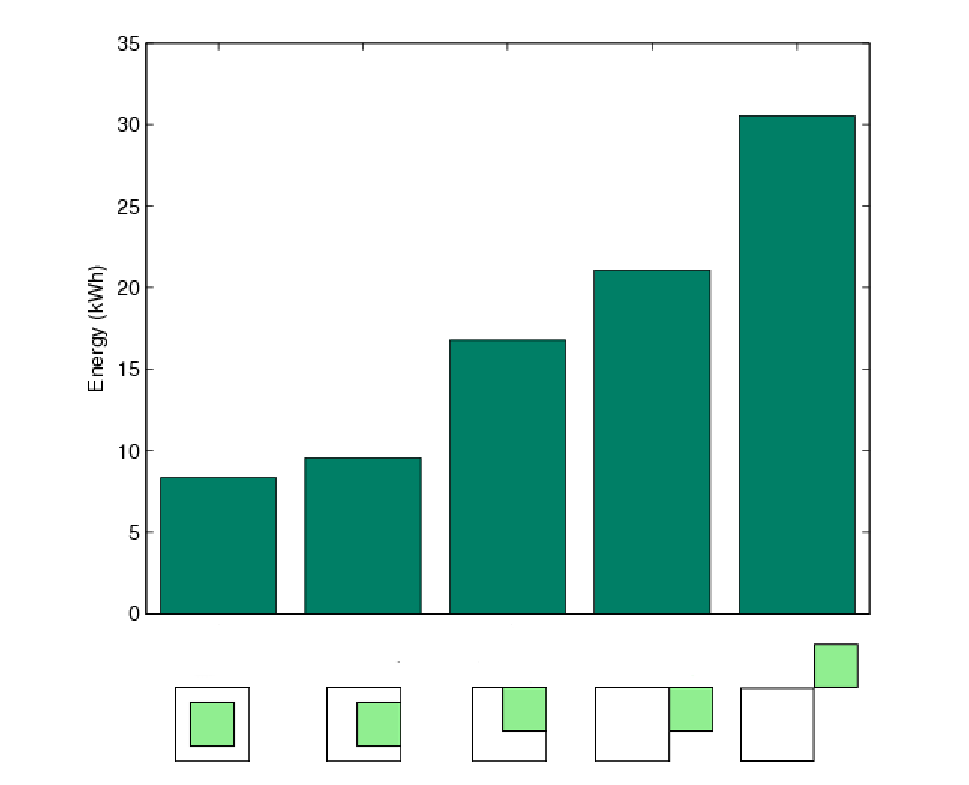
\includegraphics[width=0.55\columnwidth]{fig/wallsVsEnergyRoom}
  \caption[Effect of Exterior Walls on Energy Usage]{The energy required to
    condition a room decreases as its number of exterior walls is decreased.
    The x-axis depicts the position of the conditioned room (shaded) with
    respect to the unconditioned room (unshaded).}
  \label{fig:wallsVsEnergyRoom}
\end{figure}

\subsection{Room Occupancy}

Finally, the preliminary analysis showed that, even when a home is occupied, the
occupants use only a fraction of the house. For example, empirical analysis of
one home is shown in Figure~\ref{fig:roomUsage}, showing that primarily only one
room is used at night, three rooms are used in the evening, and four rooms are
used in the morning.

\begin{figure}[ht]
  \centering
  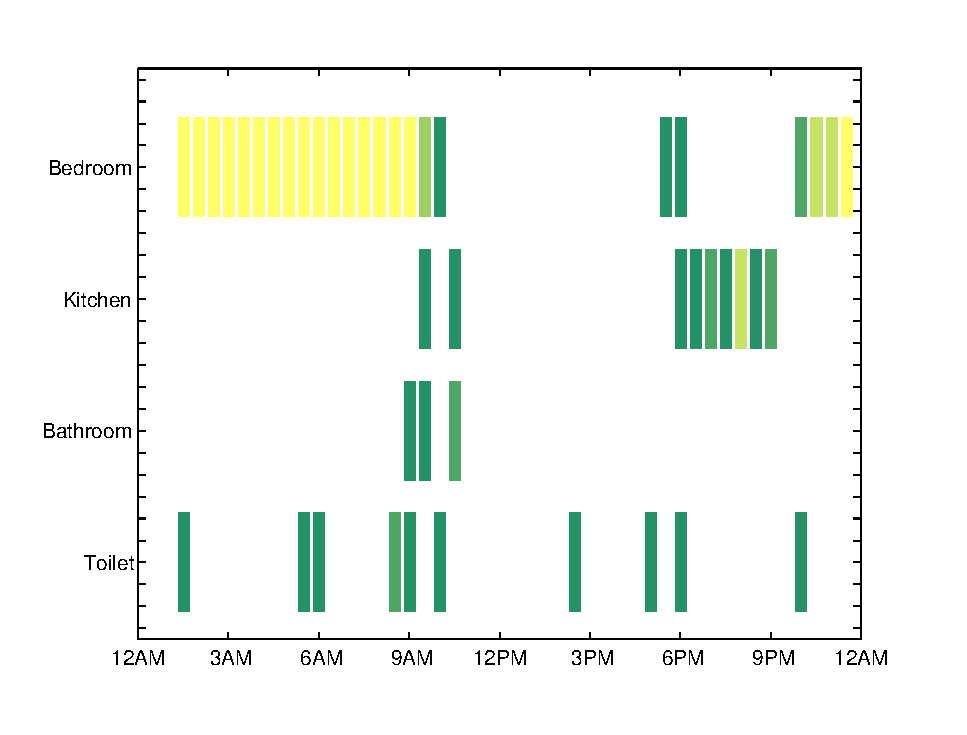
\includegraphics[width=0.6\columnwidth]{fig/roomUsage}
  \caption[Frequency of Room Usage Throughout a Day]{The frequency of room usage
    throughout a day changes. Darker colors indicate lower frequency while
    brighter colors indicate higher frequency usage with yellow being the
    highest frequency.}
  \label{fig:roomUsage}
\end{figure}

\section{Implementation}
\label{sec:implementation}

A day/night zoning system was implemented in order to empirically test the
ability to save energy with this approach. The implementation involves: (1)
sensing temperature at the room-level, (2) controlling air-flow into rooms, and
(3) controlling the HVAC system.

\subsection{Sensing House Temperature}
\label{subsec:sensingTemperature}

The home's temperature was monitored at a fine granularity by instrumenting the
house with wireless temperature sensors placed at various points on the
walls. For the deployment discussed in this section, 21 off-the-shelf
temperature sensors manufactured by La Crosse Technology~\cite{LaCrosse} were
used.  Because the temperature across the house is not uniform, one challenge in
designing a day/night zoning system is to choose how to process the temperature
readings to approximate the true average air temperature in each room.  This
problem can also be addressed for whole-house conditioning when more than a
single temperature sensor is available~\cite{lin2002multi}.

\begin{figure}[t]
  \centering
  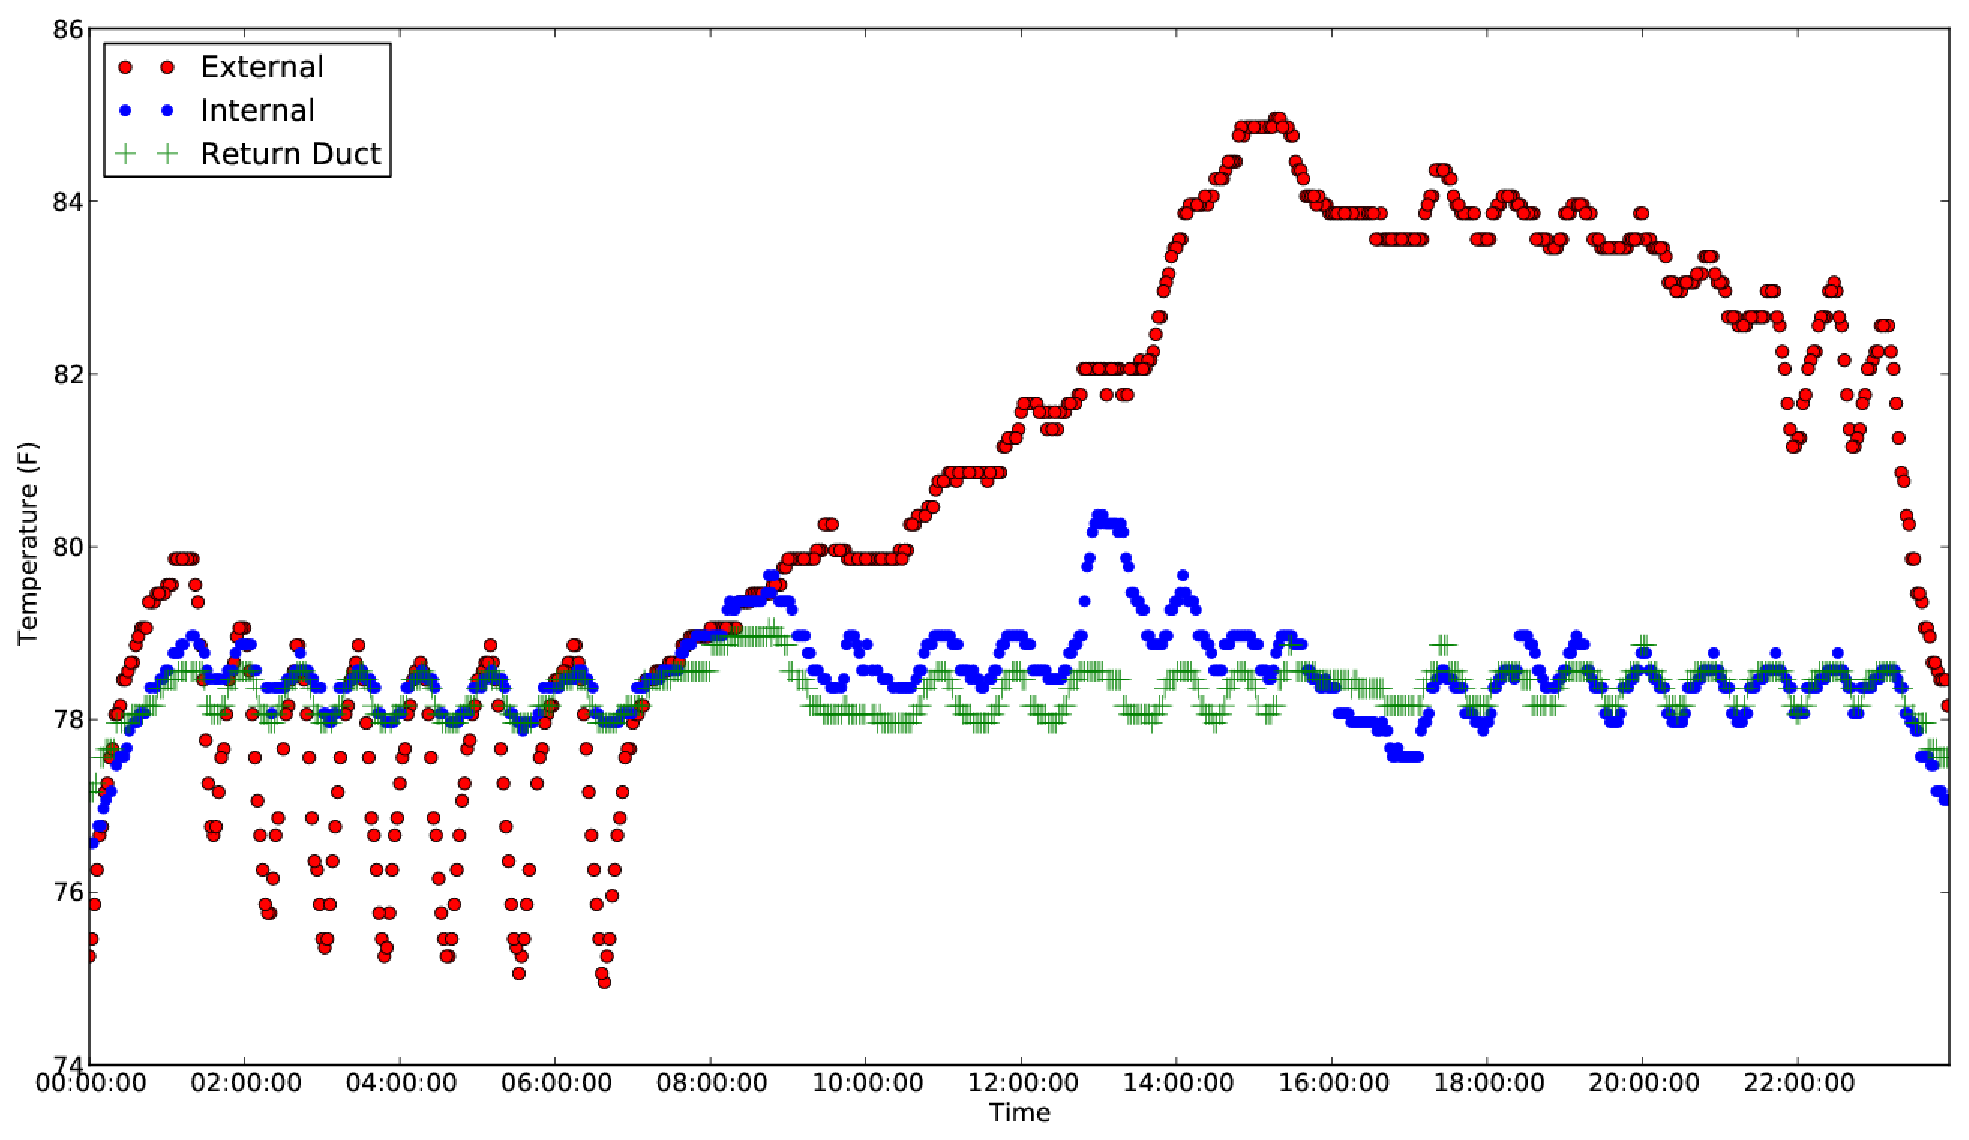
\includegraphics[width=0.6\columnwidth]{fig/intExtTherm.eps}
  \caption[Effect of Sensor Location on Temperature Reading]{The variation of
    temperature on a sensor placed on an internal wall, an external wall, and
    near the return duct.}
  \label{fig:intExtTherm}
\end{figure}

Figure~\ref{fig:intExtTherm} shows the temporal variations of several
temperature sensors placed throughout the house.  One sensor is placed in the
center of the house, directly in front of the only return register, and
therefore is exposed to a mix of air from all rooms.  Another sensor is placed
on an internal wall of the house, and a third sensor is placed on an external
wall.  The figure shows that the temperature sensor on the internal wall varies
with the temperature of the individual room, which is slightly more than the
variation of the centrally placed sensor.  However, the sensor on the external
wall is subject to wild temperature swings.  On the left side of the graph, it
is clear that the sensor has much greater downward swings than the internal
sensors.  This is because is it subject to direct air flow from the ducts, which
are typically placed on external walls.  It is also subject to heat that
concentrates around the window mid-day.  Because of these large temperature
fluctuations, only sensors on the internal walls of each room were used: the
temperature in a zone was calculated as the average of the temperatures of each
of the internal sensors in the rooms comprising the zone.

\subsection{Controlling Air-flow into Rooms}
\label{subsec:registerLeakage}

\begin{figure}[!htb]
\centering{
\subfigure[1st Generation]{
\includegraphics[width=.4\columnwidth,height=.4\columnwidth,keepaspectratio=true]{./fig/RegisterGen1Front}
\label{fig:registerGen1}
}
\subfigure[2nd Generation]{
\includegraphics[width=.3\columnwidth,height=.3\columnwidth,keepaspectratio=true]{./fig/RegisterGen2Front}
\label{fig:registerGen2}
}
\subfigure[3rd Generation]{
\includegraphics[width=.3\columnwidth,height=.3\columnwidth,keepaspectratio=true]{./fig/RegisterGen3}
\label{fig:damper}
}
\subfigure[Bench-Top Test Rig]{
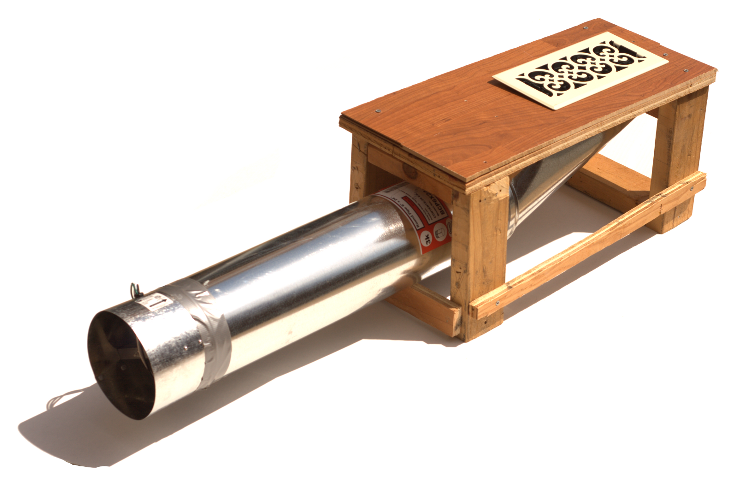
\includegraphics[width=.3\columnwidth,height=.3\columnwidth,keepaspectratio=true]{./fig/testRig}
\label{fig:testRig}
}
\caption[Three Generations of Active Registers and Bench-Top Test Rig]{(a)
Version 1 uses servo motors and a rotating louver design, but exhibited too much
leakage.  (b) Version 2 uses a sliding gate design to solve the leakage
problems, but causes too much noise.  (c) Version 3 is a commercial in-line
damper with a servo motor used for traditional zoning applications. (d) The
bench-top test rig used to verify that the second generation wirelessly
controlled active registers have almost no air leakage.}
\label{fig:activeRegisters}
}
\end{figure}

In order to control the airflow into individual rooms {\em active registers and
dampers} that can be wirelessly opened or closed were designed and built. While
controllable registers are commercially available, they actuate based on either
preset temperatures or temporal schedules. Commercial active registers that are
controllable through a remote control would be hard to integrate with the
day/nigh zoning's wireless control system and such registers are expensive,
costing over \$50 each. By retrofitting passive registers with servo motors,
active registers were obtained for under \$20 each, excluding the cost of the
radio and microcontroller. These registers integrated wirelessly with the rest
of the Dual-Zone infrastructure. The active register design improved
through three generations as shown in Figure~\ref{fig:activeRegisters}. The
registers were implemented using commercial, off-the-shelf (COTS) components
including an operable register, a servo motor, and a small amount of custom
circuitry (Figure~\ref{fig:activeRegister}).  These components resulted in a
cost of less than \$20 per register excluding the cost of the TelosB mote, which
was used for wireless communication. These registers were inspired by several
prototypes and even commercial versions of similar hardware that are currently
available~\cite{walker2003register,walker2008residential,watts2007application,TRANE2003},
but go beyond these devices by integrating them into a cooperative, wireless
system.

\begin{figure}[!htb]
  \centering{
    \subfigure[Wireless Controller]{
    \includegraphics[width=.4\columnwidth]{./fig/registerBack}
      \label{fig:registerBack} }
    \subfigure[Face Plate of Active Register]{
    \includegraphics[width=.4\columnwidth]{./fig/registerFront}
    \label{fig:registerFront} } } \caption[Details of an active register]{A
    wirelessly controlled active register built by augmenting a standard vent
    register with a TelosB mote and a servo motor.} 
\label{fig:activeRegister}
\end{figure}

The effectiveness of the registers were measured using the bench-top testing
framework shown in Figure~\ref{fig:testRig}. The first generation registers were
not very efficient at blocking air when closed. The second generation registers
improved this aspect by blocking nearly 100\% of airflow but was noisy when
opening and closing. Due to these reasons dampers used in commercially
implemented zoned systems were used as the third generation of airflow
controllers.

\begin{figure}[!htb]
  \centering
  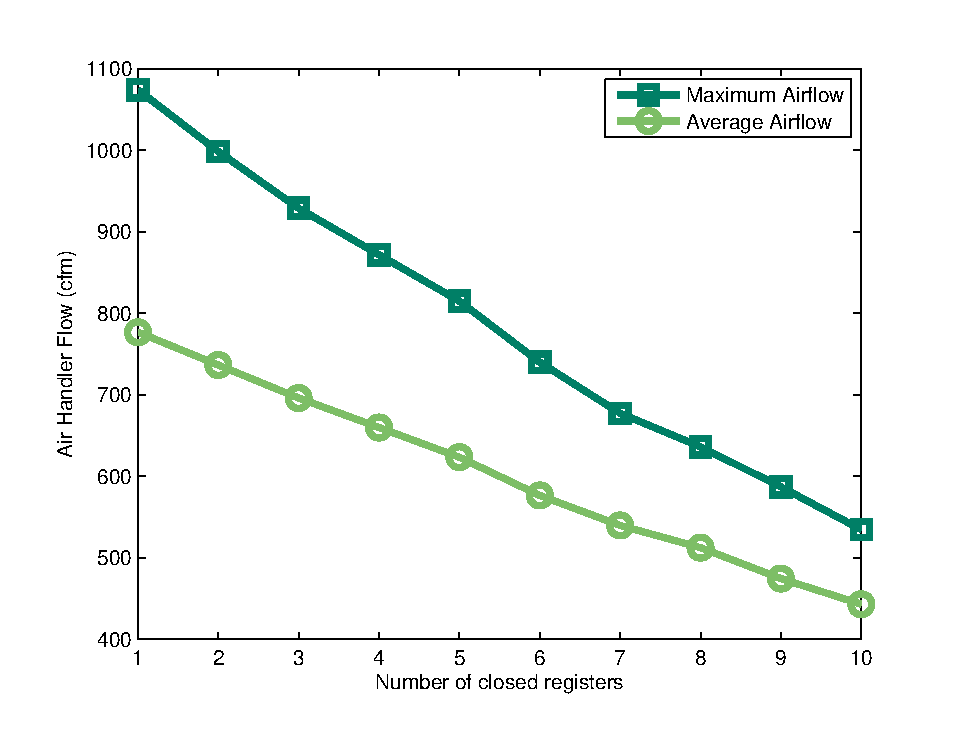
\includegraphics[width=0.6\columnwidth]{fig/regClosingAirflow.eps}
  \caption[Effect of Closing Registers on Air Flow]{As more registers are
    closed, some efficiency is lost and the total total air volume output by the
    system decreases.}
  \label{fig:regClosingAirflow}
\end{figure}

The effectiveness of these registers at directing airflow into different rooms
was measured using a Kestrel 4100 Pocket Air Flow Tracker manufactured by
Nielsen-Kellerman~\cite{kestrel}. This sensor is placed above the register and
provides a measure of airflow in terms of cubic feet per minute (CFM) that is
coming out of the register.  This measurement is based on the known size of the
register and the speed of the air.  Figure~\ref{fig:regClosingAirflow} shows
that the total airflow coming from all registers is reduced as an increasing
number of registers are closed.  When all registers are open, the average
airflow is approximately 800 CFM, which matches the specification of the air
handler in this house.  However, as more registers are closed, the average
airflow approaches 450 CFM, which is almost half. Total airflow does not
approach zero because some air escapes even from the closed registers.  This
result verifies that closing registers does decrease the overall efficiency of
the system because it reduces the total airflow output, as suggested
by~\cite{walker2003register}.  Therefore, actively cooling only half the house
would not cause double the amount of air to be available to the cooled zone,
because some air is lost due to backpressure, increased duct friction, duct
leakage, and leakage from the closed registers.

\subsection{Controlling the HVAC System}
\label{subsec:controllingHVAC}

\begin{figure*}[!htb]
  \centering
  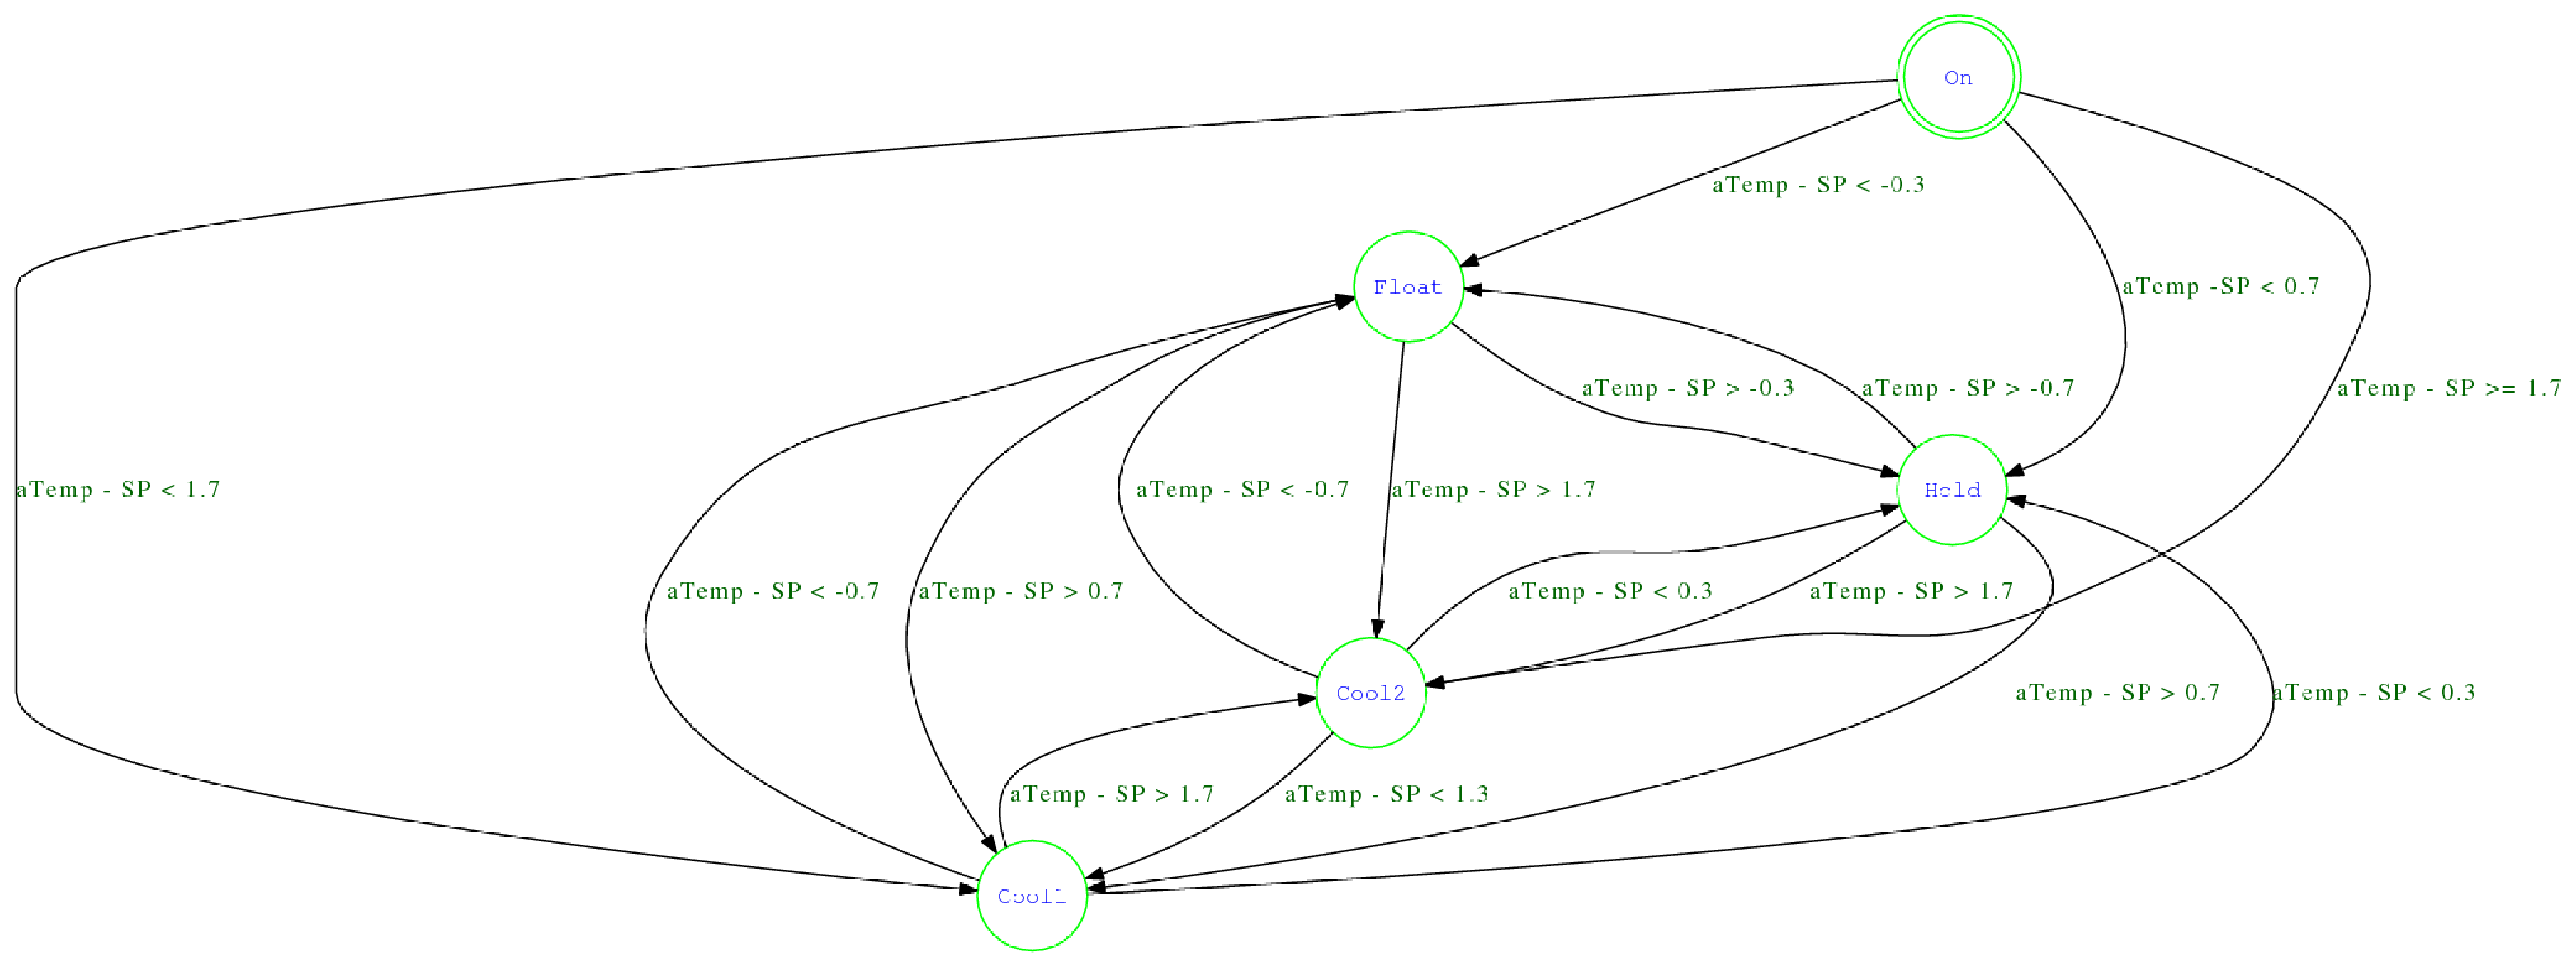
\includegraphics[width=1.0\columnwidth]{fig/fsm.eps}
  \caption[Finite State Machine of Dual-Zone Controller]{The
  zoning controller attempts to maintain the average temperature of the active
  zone (aTemp) at the desired setpoint (SP) by transitioning the system between
  five states.}
  \label{fig:stateMachine}
\end{figure*}

Dual-Zone uses a simple state machine (Figure~\ref{fig:stateMachine}) to
control the HVAC system through four possible stages: {\em Float}, {\em Hold},
{\em Cool 1}, and {\em Cool 2}. Cool 1 and Cool 2 are intended to represent
different stages of the HVAC system in which the compressor and hair handler
operate at different cooling capacities.  Hold causes the HVAC system to
maintain the current temperature at the thermostat, and Float causes the HVAC
system to turn off.

\begin{table}[htp]
  \centering
  \begin{tabular}{|c|l|}
    \hline
    \small State & \small ~~~~~~~~~~~~~Action\\
    \hline
    \small Float & \small ThermSP = ThermTemp + 1 \\
    \small Hold & \small ThermSP = ThermTemp \\
    \small Cool1 & \small ThermSP = ThermTemp - 1 \\
    \small Cool2 & \small ThermSP = ThermTemp - 2 \\
    \hline
  \end{tabular}
  \caption[Coarse-grained abstraction for thermostat operation]{The operating stage of the HVAC equipment was controlled by adjusting the thermostatic setpoint {\em
  ThermSP} with respect to the temperature that was sensed by the thermostat {\em ThermTemp}.}
  \label{table:abstraction}
\end{table}

In order to control the HVAC equipment, the Dual-Zone controller must
interface through an Internet-controllable thermostat manufactured by
BAYweb~\cite{bayweb}. However, the BAYweb thermostat only allows its setpoint to
be changed; it does not allow direct control over the equipment. In order to
control the equipment, therefore, the setpoint of the thermostat $ThermSP$ was
modified to be higher, lower, or equal to the temperature measured at the
thermostat $ThermTemp$.  When the equipment needed to be put into the {\em
float} state, a setpoint that is higher than the current temperature was used.
This causes the thermostat to turn off the equipment.  Similarly, when it was
necessary to hold or lower the temperature, a setpoint that is the same as or
lower than the current temperature, respectively, was used.  To lower the
temperature quickly, i.e. to use stage {\em Cool 2}, a setpoint that is two
degrees lower than the setpoint was used.  This exploits the PI controller that
is built into the thermostat, which causes the equipment to go into high stage
cooling when the temperature is two degrees from the setpoint for more than 5
minutes.  The operation of the system is summarized in
Table~\ref{table:abstraction}.  This coarse-grained control over the equipment
is not ideal and could have caused some loss of efficiency and energy waste.  In
case study 2~\ref{ch:cs2} a custom thermostat is built to provide finer grained
control that produced better results

\subsection{Software Implementation}

Dual-Zone was deployed in an 8-room, single story, 1200 square foot residential
building shown in Figure~\ref{fig:cs1Floorplan}.  For simplicity, the house was
divided into two zones.  The red zone composed of the living room, dining room,
and kitchen is actively conditioned between 8:00 AM and 9:30 PM while the blue
zone composed of the bedroom, nursery, toilet, and mudroom is conditioned
between midnight and 8:00 AM. Between 9:30 PM and midnight the whole house is
conditioned. This approach is compared to conditioning of the whole house using
an off-the shelf programmable thermostat manufactured by {\em
BAYweb}~\cite{bayweb}.  In both cases, the setpoint temperature of the house is
controlled by the occupants. This means that the experiments measure the energy
required to keep the occupants comfortable with both systems, as opposed to
keeping the space at a particular setpoint.

\begin{figure}[ht]
  \centering
  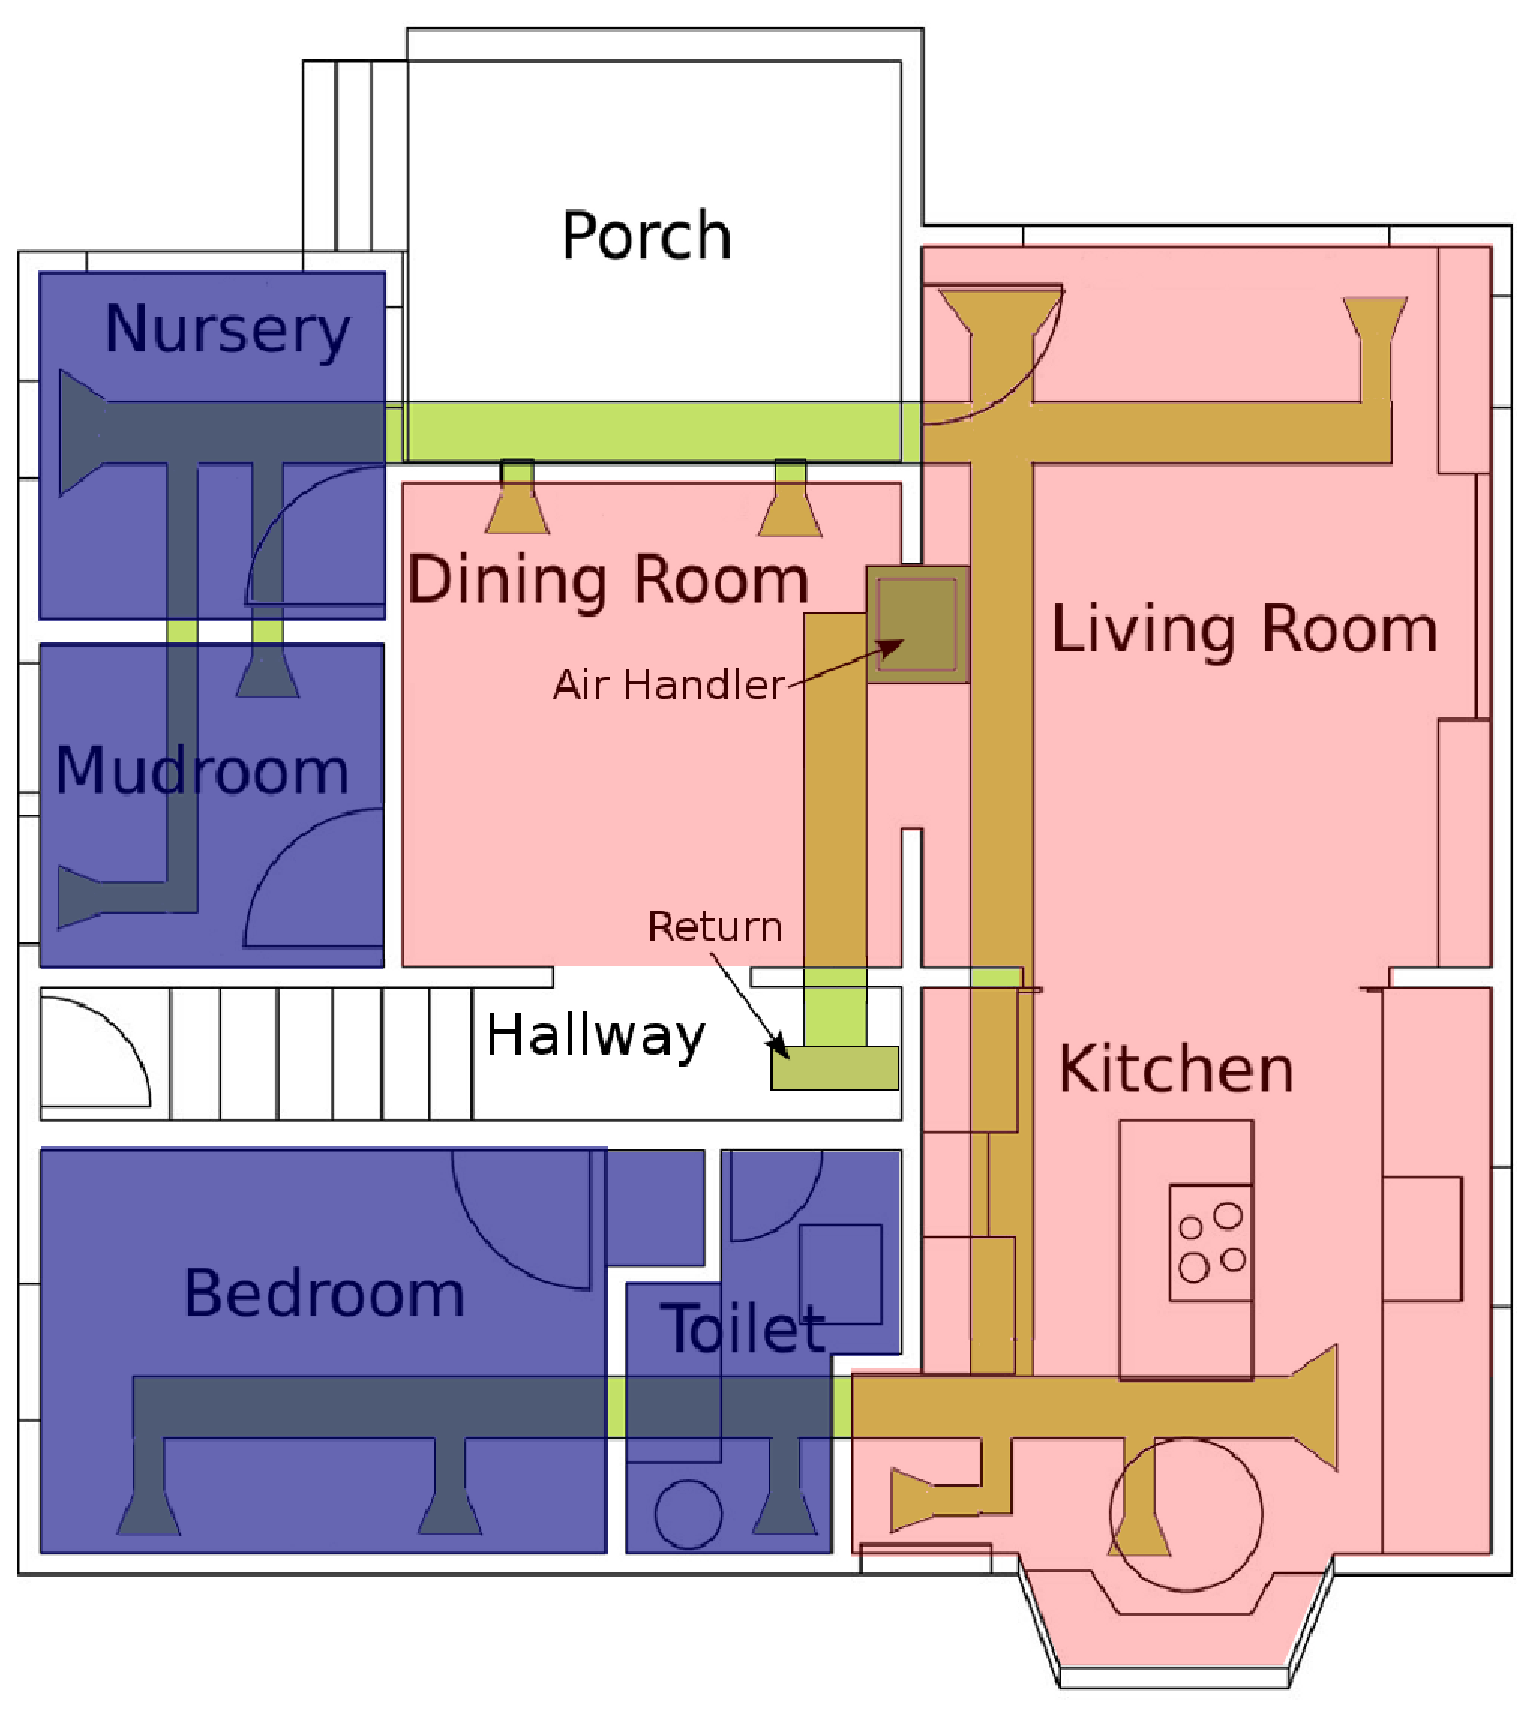
\includegraphics[width=0.6\columnwidth]{fig/floorplan-mechanicalZoned.eps}
  \caption[The residential testbed used for zoning studies]{The residence in
  which experiments were carried out with green ducts terminating in registers
  that can be opened or closed. The rooms that compose the day zone are shaded
  in light red and the rooms that compose the night zone are shaded in dark
  blue. The red circles show locations of some of the temperature sensors used
  for HVAC control.}
  \label{fig:cs1Floorplan}
\end{figure}

The software that controlled the system was written using Python. Due to the
fact that the MacroLab function libraries and hardware drivers are very
immature, and it would have taken a considerable about of time and effort to
incorporate the required function into the library, the actual implementation
was done only in Python. The programs written in Python read from the
temperature and motion sensors and sent actuation commands to active registers
and the HVAC hardware. Figure~\ref{fig:stateMachine} presents a state machine of
the controller that was implemented in Python. The controller transitions the
HVAC system between the four states listed in Table~\ref{table:abstraction}
depending on the current state, the average temperature ({\em aTemp}) in the
active zone and the setpoint ($SP$) using hysteresis to prevent rapid
fluctuations between states. This program was executed to collect the data used
to analyze Dual-Zone.

\begin{figure}[!htb]
  \begin{macrolab}
RTS = RunTimeSystem();
weatherdirect = RTS.getMotes('type', 'weatherdirect');
tempSensors = SensorVector(weatherdirect, 'temperature');
x10 = RTS.getMotes('type', 'X10');
motionSensors = SensorVector(x10, 'motion');
zones = uint8({[3 4 5], [1 2 6 7]}); % Day/Night zones
motionSensorIDs = uint8({[8 1 9], [2 6], [10 5], [4], [7 11], [12 14], [3 15]});
tempSensorIDs = uint8({[1 3], [2], [6 7], [4 9 11], [12 13], [5 14], [8 10]}); 
nightStart = [0 0 0 2 0 0];
nightEnd = [0 0 0 7 0 0];
curState = 'On'
every(60000)
  mode = dbRead('zoning', 'mode', 'latest')
  motionVals = motionSensors.sense();
  tempVals =  tempSensors.sense();
  curTime = clock;
  curNightStart = nightStart;
  curNightStart(1:3) = curNightStart(1:3) + curTime(1:3);
  curNightEnd = nightEnd;
  curNightEnd(1:3) = curNightEnd(1:3) + curTime(1:3);
  curZone = {};
  if datenum(curTime) <= datenum(curNightStart) && datenum(curTime) > datenum(curNightEnd)  
    curZone = zones{1};
  else
    curZone = zones{2};
  end
  curZoneMotion = [];
  curZoneTemps = [];
  for room = curZone
    curZoneMotion = [curZoneMotion motionVals(motionSensorIDs{room})];
    curZoneTemps = [curZoneTemps tempVals(tempSensorIDs{room})];
  end
  if sum(curZoneMotion) > length(curZoneMotion) / 2
    SP = dbRead('zoning', 'setpoint', 'latest');
  else
    SP = dbRead('zoning', 'setback', 'latest');
  aTemp = mean(curZoneTemps);
  if mode == 'heat'
    deltaTemp = SP - aTemp;
  else
    deltaTemp = aTemp - SP;
  end
  curState = getNextState(curState, deltaTemp);

  hvacActuate(mode, curState, curZone);
end
  \end{macrolab}
  \smallskip
  \hrule width 1\columnwidth
  \caption{MacroLab implementation of Dual-Zone.}
  \label{code:cs1}
\end{figure}

As a case study, the Dual-Zone controller software was re-implemented using
MacroLab as shown in the code in Figure~\ref{code:cs1}. The MacroLab
implementation is based on the temperature and motion sensor reading being
abstracted as macrovectors that can be indexed using room IDs. Actual usage of
this program to control Dual-Zone would require the implementation of two driver
functions: $dbRead$ to read from a database and $hvacActuate$ to actuate the
HVAC system and active registers. This code could execute with the COTS sensors
used to implement Dual-Zone by providing implementations of $weatherDirect$ and
$X10$ that read sensor values from the Weather Direct web interface and X10 base
station or query the appropriate database tables. If other sensors, such as
SnapPys or motes, that could be programmed were used for sensing instead, sensor
driver implementations that push, or aggregate, data could be used to optimize
the execution of this code by just replacing the $type$ parameter in the
$getMotes$ function as described in
Section~\ref{sec:cs1macroprogrammingDiscussion}.

\begin{figure}[!htb]
  \begin{macrolab}
function getNextState(curState, deltaTemp)
  if curState == 'On'
    if deltaTemp < -0.3
      curState = '-1'; % float
    elif deltaTemp < 0.7
      curState = '0'; % hold
    elif deltaTemp < 1.7
      curState = '1'; % heat/cool 1
    elif deltaTemp >= 1.7
      curState = 2; % heat/cool 2
  elif state == '-1'
    if deltaTemp > -0.3
      curState = '0';
    elif deltaTemp > 0.7
      curState = '1';
    elif deltaTemp > 1.7
      curState = '2'; 
  elif state == '1'
    if deltaTemp < -0.7
      curState = '-1';
    elif deltaTemp < 0.3
      curState = '0';
    elif deltaTemp > 1.7
      curState = '2';
end
  \end{macrolab}
  \smallskip
  \hrule width 1\columnwidth
  \caption{MacroLab function to calculate transition in hysteresis state
  machine.}
  \label{code:getNextState}
\end{figure}

\section{Evaluation}
\label{sec:evaluation}

To evaluate Dual-Zone the control of the HVAC system is alternated between
single-zoned whole house control and day/night zoned control over a twenty day
period, such that each system ran every other day. This experimental procedure
was selected to minimize the effect of changing weather patterns on energy
statistics. Both systems executed for a total of 10 days. The energy consumed by
all systems in the house was monitored using The Energy Detective
(TED)~\cite{Energy} real-time in-home energy management system and the amount of
energy used by the HVAC system was deduced using the operation logs generated by
the BAYweb thermostat.


\subsection{Zoning Evaluation}

Figure~\ref{fig:energyBoxplot} shows the energy consumed in conditioning a house using
Dual-Zone and whole house conditioning. This graph indicates that whole-house
conditioning consumed 20.5\% more energy than the prototype implementation of
Dual-Zone, on average.

\begin{figure}[!htb]
  \centering
  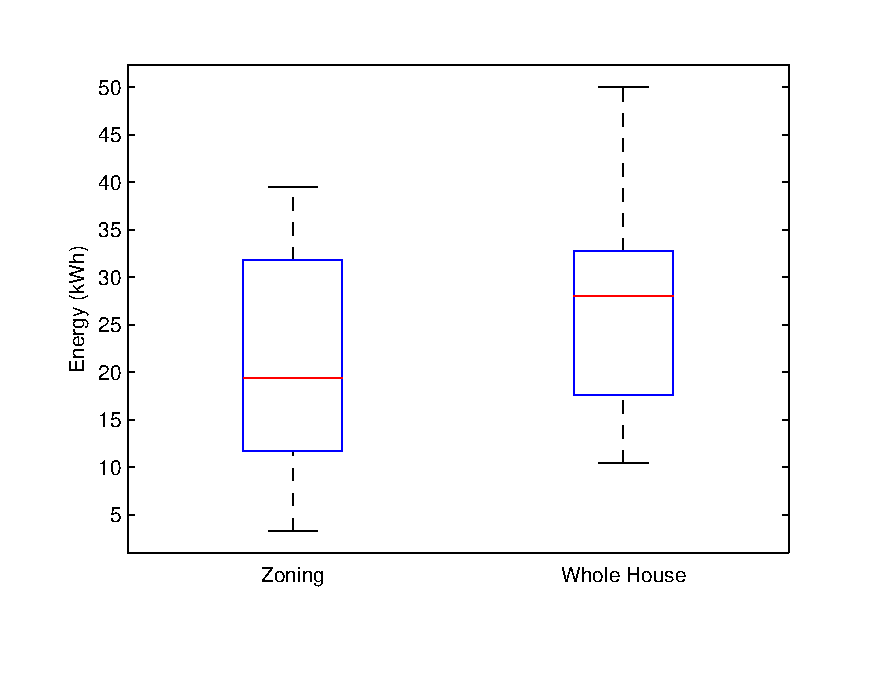
\includegraphics[width=0.6\columnwidth]{fig/cs1boxplot.eps}
  \caption[Energy usage of day/night zones vs. whole house conditioning]{The
  implementation of Dual-Zone uses 20.5\% less energy than whole house
  cooling on average.}
  \label{fig:energyBoxplot}
\end{figure}

Figure~\ref{fig:energy} shows the actual energy consumption for each day as a
scatter plot, with the average temperature of for that day on the x-axis, the
energy consumed on the y-axis, and the control algorithm shown as the color of
the scatter point.

\begin{figure}[!htb]
  \centering
  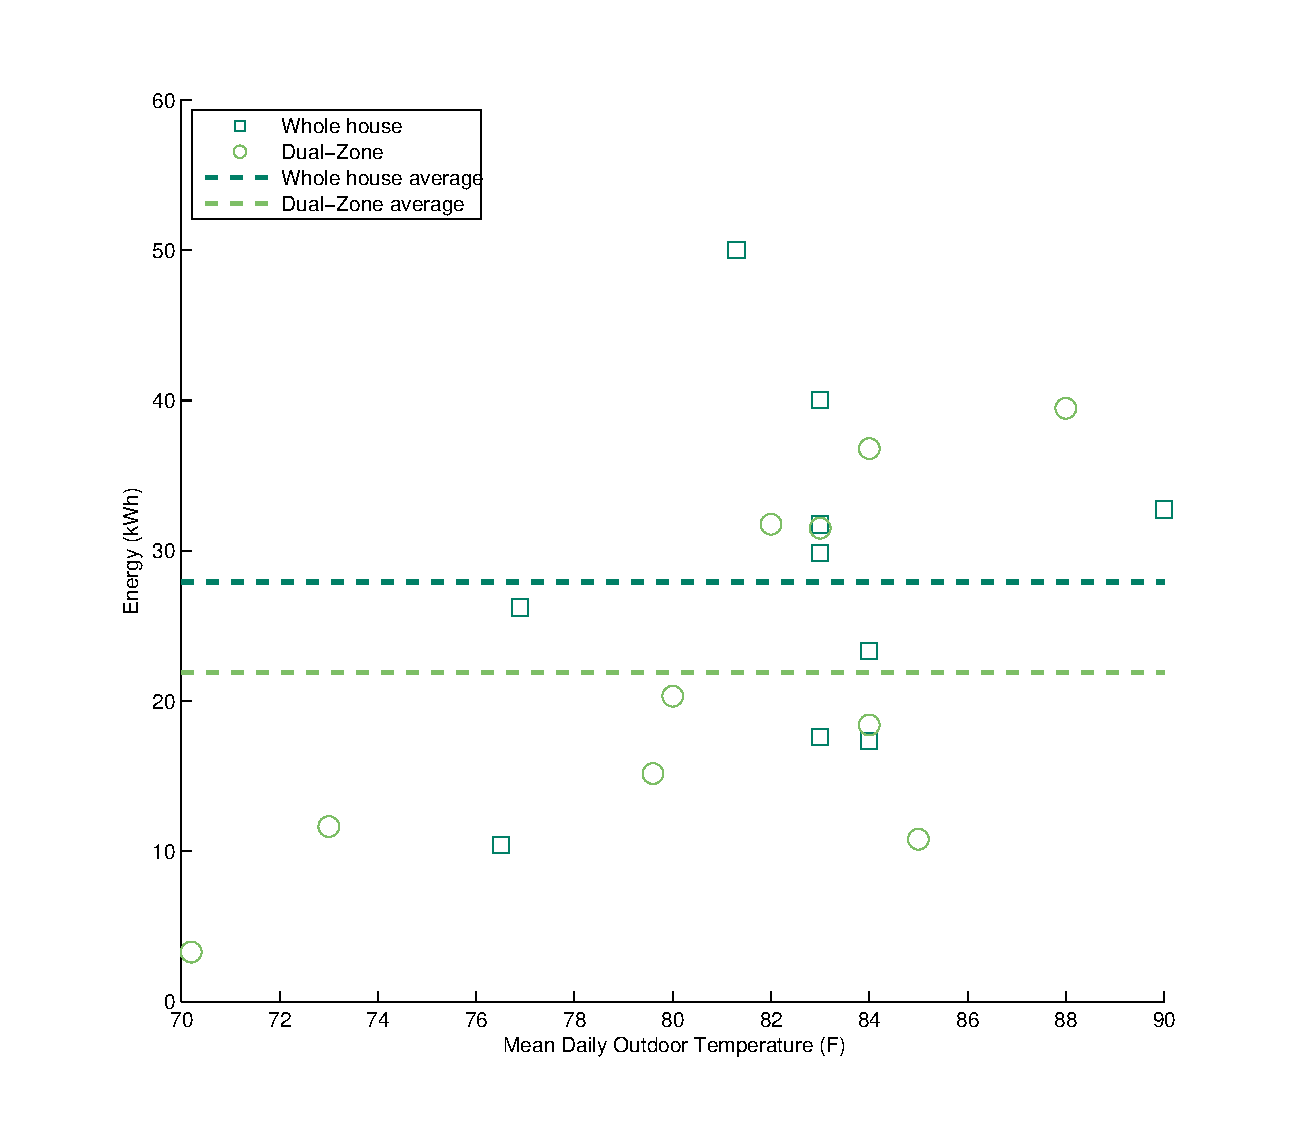
\includegraphics[width=0.6\columnwidth]{fig/meanEnergyScatter.eps}
  \caption[Effect of outdoor temperature on energy usage]{The dotted lines
  indicate the average energy used over the experimental period.}
  \label{fig:energy}
\end{figure}

Figure~\ref{fig:houseTempRes} shows how the temperature of several rooms in
different zones vary as the temperature in the active zone was dropped from 76
to 72 degrees.  In this graph, the bottom three lines shown the temperature of
conditioned rooms over time while the top two lines show the temperature of
unconditioned rooms.  Although some leakage is evident, particularly into the
top line, the temperatures of the unconditioned rooms remains substantially
higher than the conditioned rooms.  These temperature traces explains how
Dual-Zone is able to save energy by reducing the size of the space that
must be conditioned.

\begin{figure}[ht]
  \centering
  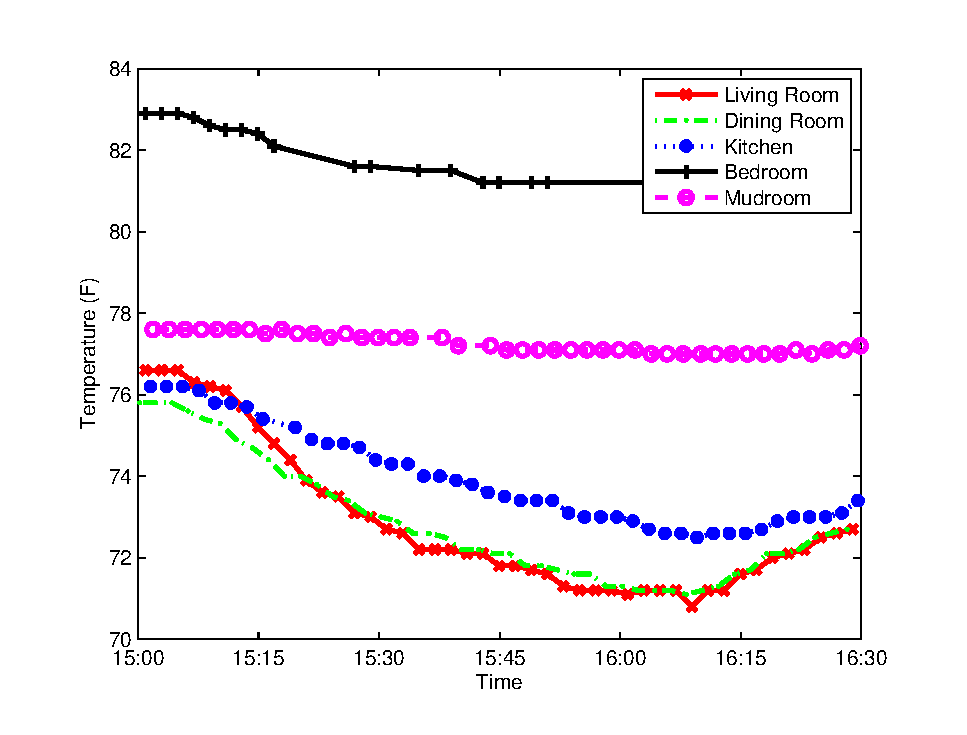
\includegraphics[width=0.6\columnwidth]{fig/houseTempRes.eps}
  \caption[Temperature Response of Conditioned and Unconditioned
  Rooms]{Temperature response of both conditioned and unconditioned rooms as the
  active zone temperature is dropped from 76 to 72.}
  \label{fig:houseTempRes}
\end{figure}

In order to better understand these results, Figure~\ref{fig:airflowBar}
illustrates how effective the active registers were at activating and
de-activating the red and blue zones.  It is clear from this figure that the
greatest airflow in a zone is obtained when the registers in the other zone are
closed.  However, air flow to the inactive zone does not stop, nor does it all
get directed to the active zone. In future work, the active register system
needs to be improved to produce better energy saving and thermal insulation
results.

\begin{figure}[ht]
  \centering
  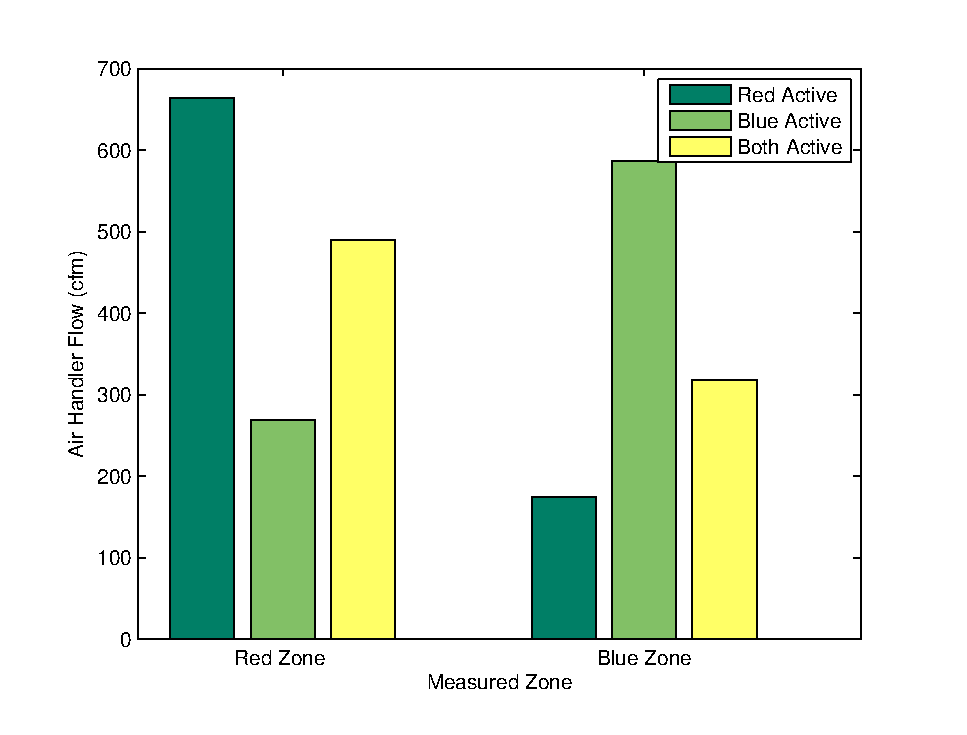
\includegraphics[width=0.6\columnwidth]{fig/airflowBar.eps}
  \caption[Effect of Zoning on Airflow]{Activating different zones does not
    redirect all air flow from one zone to another, but does affect air flow
    substantially.}
  \label{fig:airflowBar}
\end{figure}

\subsection{Macroprogramming Discussion}
\label{sec:cs1macroprogrammingDiscussion}

For case study 1, MacroLab proved to be a much more convenient language in which
to program than Python. The Dual-Zone controller presented in
Figures~\ref{code:cs1} and~\ref{code:getNextState} is written in fewer than 100
lines of MacroLab code. Making a conservative estimate of 200 lines of code with
the addition of low-level functionality, such as hardware drivers, implementing
Dual-Zone in MacroLab is much more efficient in terms of code size
compared to the over 500 lines of code written for the Python implementation. An
added advantage of MacroLab is the ability for the run-time system (RTS) to
automatically optimize the code based on available hardware or the topology of
the network. The following subsections describe some of the optimizations that
would have been possible with a MacroLab implementation of Dual-Zone.

\subsubsection{In-Network Data Processing}
In the implementation of Dual-Zone using Python, all temperature sensors
transmitted readings periodically. By providing the MacroLab RTS with
$tempsensor.sense$ and $motionsensor.sense$ functions that are aware of a
sensor's location and the current time, node-level code could be generated where
sensors only transmit their temperature or motion readings if they are in the
currently active zone. In essence, the following portion of the macroprogram is
pushed into the network, to be executed at the sensors rather than the base
station.

\begin{macrolab}
if datenum(curTime) <= datenum(curNightStart) && datenum(curTime) > datenum(curNightEnd)  
  curZone = zones{1}
else
  curZone = zones{2};
end
curZoneMotion = []
curZoneTemps = []
for room = curZone
  curZoneMotion = [curZoneMotion motionVals(motionSensorIDs{room})]
  curZoneTemps = [curZoneTemps tempVals(tempSensorIDs{room})]
end
\end{macrolab}

This simple optimization could almost halve the number of
messages sent by a sensor, potentially doubling their battery life. For
temperature sensors which have an average lifetime of a year, an increase
to two years is very beneficial. 

\subsubsection{In-Network Aggregation}
Another optimization that MacroLab could enable is in-network aggregation. Each
of the two zones could form independent neighborhoods with an aggregation tree
built from the furthest sensors towards the base station. The average
temperature of the zone could be aggregated by each sensor calculating the sum
of its and its children's temperatures and passing it up the tree along with a
count of the number of temperatures that were summed. The base station would
receive a temperature sum from the zone along with the total number of sensors
within the zone, which can be used to calculate the average temperature of the
zone. Without in-network aggregation, for a set of $N$ sensors where sensor $i$
is at a depth of $d_i$ from the base station, the number of messages transmitted
each time is $\displaystyle\sum\limits_{i \in N} d_i$. Using in-network
aggregation reduces the number of messages sent to equal the number of sensors
in the network, $N$. In-network aggregation only proves beneficial if the system
involves a multi-hop network since in a single-hop network all transmissions can
be received at the base station where computation could be carried out centrally.

\subsubsection{Data Fusion}
Finally, the MacroLab RTS could use data fusion to minimize the number of
messages passed to the base station by aggregating the motion sensor and
temperature sensor values at a leader node within each zone. The leader node
would execute the following portion of the macroprogram:

\begin{macrolab}
if sum(curZoneMotion) > length(curZoneMotion) / 2
  SP = dbRead('zoning', 'setpoint', 'latest');
else
  SP = dbRead('zoning', 'setback', 'latest');
aTemp = mean(curZoneTemps);
if mode == 'heat'
  deltaTemp = SP - aTemp;
else
  deltaTemp = aTemp - SP;
end
\end{macrolab}

By processing both the temperature and motion sensor data within the network,
the number of messages passed by both sensors up to the base station can be
minimized. This approach provides savings only for very large networks where all
the nodes in a particular zone are multiple hops from the base station. The RTS
can optimize this further by keeping track of the previous $deltaTemp$ value and
only transmitting a $deltaTemp$ value if the new value exceeds the previous
value by a threshold.

\section{Conclusions}
\label{sec:conclusions}

This study demonstrates how MacroLab can be used to simplify the software
implementation of a static day/night zoning system. It also shows the power of
deployment-specific code decomposition (DSCD) in optimizing an application to
suit network topologies and available hardware. The case study involves
minimizing the energy consumed for heating and cooling homes by conditioning
only occupied spaces. The implementation of Dual-Zone shows that a
centralized HVAC system can be cheaply and easily retrofitted to save
energy. Even with leakage from the registers and imperfect isolation between
rooms, whole house zoning consumed 20.5\% more energy than this system over the
course of a 20-day study.  While longer-term studies are necessary to eliminate
potential effects of weather during the study, these results are promising and
warrant further investigation into this approach, especially in light of the
shortcomings of the prototype, as described in Section~\ref{sec:implementation},
and the fact that only multi-room zones were evaluated instead of room-level
zones. Case study 2~\ref{ch:cs2} builds on Dual-Zone to implement a
room-level zoning system which is used to show how the evolution of software is
simplified by MacroLab and the limitations of macroprogramming abstractions as
system complexity increases.
